\documentclass[1]{report}
\usepackage[utf8]{inputenc}
\usepackage[T1]{fontenc}
\usepackage[francais]{babel}
\usepackage{listings}
\usepackage{hyperref}
\usepackage{graphicx}
\usepackage{subcaption}
\usepackage{caption}
\usepackage{xcolor}
\usepackage{sectsty}
\usepackage{algorithm}
\usepackage{algorithmic}
\usepackage{titlesec}

\hypersetup{ %Paramètres pour les liens hypertextes
	colorlinks=true,
	linktoc=all,
	linkcolor=blue,
	urlcolor=blue,
}

\title{\textcolor{red}{Projet KenKen2 : Mémoire}}
\author{Erwan Dupland, Sébastien Granger, Hugo Jalenques, Pablo Tomas
\\ Client : Emmanuel Fleury \\ Chargé de TD : Simon Archipoff}
\date{Rendu du 04 Avril 2019}

\begin{document}


  
\chapterfont{\color{black}}

\maketitle

\renewcommand{\contentsname}{Sommaire} 
\tableofcontents

\chapter{Introduction}


		Le but de ce projet est de concevoir un programme capable de résoudre et de générer des grilles pour le jeu KenKen. \newline
		
		Selon Wikipedia : \newline
		
        \textit{Le KenKen ou kendoku est un jeu mathématique dérivé du sudoku créé par un instituteur japonais, Tetsuya Miyamoto.}
        
        \textit{
        Dans le cadre de son enseignement, Tetsuya Miyamoto a conçu des exercices pour ses élèves en forme de grilles de jeu dans le but de les aider à apprendre et à réviser leurs bases de calcul tout en s'amusant.
        Face à l'enthousiasme de ses élèves, il a imaginé différents niveaux de difficulté, différents niveaux qui ont permis à ses grilles KenKen de rencontrer un certain succès au Japon.}
        
        \textit{
        Le jeu consiste à compléter une grille par des chiffres en les trouvant par déduction ou par calcul.}
        
        \textit{
        Le KenKen est donc une grille de chiffres à compléter. On peut aisément rapprocher ce jeu du jeu sudoku, en effet, il mêle intuition, jeu de logique et jeu de calcul.}
        
        \textit{
        Comme pour le sudoku, le but du jeu est de remplir toutes les cases de la grille avec des chiffres allant de 1 à n (n étant la taille de la grille KenKen, autrement dit, le nombre de lignes et de colonnes dans la grille) sans jamais avoir deux fois le même chiffre dans la même colonne ou sur la même ligne.}
      

\chapter{Définitions des termes du KenKen}

Dans le but de clarifier certaines notions que nous jugeons essentielles, nous allons dans cette partie, définir chacun des termes spécifiques au Kenken que nous employons tout au long de ce rapport.\par

    \section{Case}
    
    \begin{figure}[h]
    \centering
        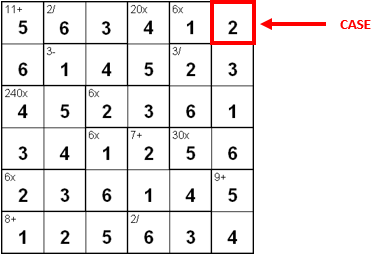
\includegraphics[scale=0.9]{case.PNG}
        \caption{Case}
    \end{figure}
    
    Au début d’une partie, toutes les cases sont vides. Le joueur doit remplir les cases vides en respectant certaines règles pour terminer la partie.
    
    Une case, qu’elle soit vide ou remplie, appartient à un seul bloc. Cette case peut aussi contenir une contrainte.
    
    \section{Bloc}
  
    
    Un bloc désigne la zone d'application d'une contrainte. Un bloc contient au minimum une case et ne peut pas dépasser la taille de la grille.
    
    \begin{figure}[H]
    \centering
        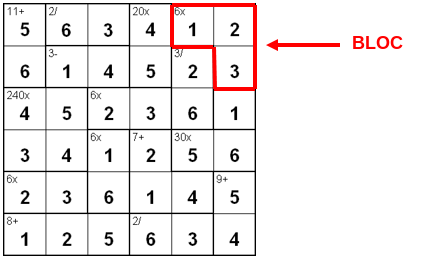
\includegraphics[scale=0.5]{bloc.png}
        \caption{Bloc}
    \end{figure}  
    
    \section{Contrainte, cible et opérateur}
    
  
    
    Une contrainte se trouve dans une case qui elle-même se trouve à l’intérieur d’un bloc. \newline

    Les contraintes sont une spécificité du jeu KenKen, en effet il va falloir atteindre la cible spécifiée par la contrainte en effectuant une opération sur toutes les cases d'un même bloc.
    
    Les opérations possibles dans une grille KenKen sont l’addition, la soustraction, la multiplication et la division.
    

      \begin{figure}[H]
    \centering
        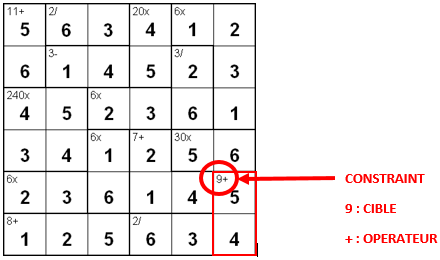
\includegraphics[scale=0.9]{constraint.PNG}
        \caption{Une contrainte d'opérateur + et de cible 9}
    \end{figure}
     
    
    En ce qui concerne les cas de la soustraction et de la division, il n’y a pas d'ordre obligatoire à respecter pour remplir les blocs. \newline
    
    Ainsi :

    \begin{figure}[h]
    \centering
        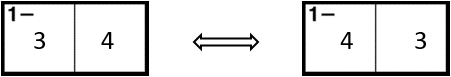
\includegraphics[scale=0.9]{ordre_contrainte.PNG}
        \caption{Ordre des valeurs}
    \end{figure}
    
    Ces deux blocs respectent bien la contrainte qui est d’obtenir 1 en soustrayant les deux cases du bloc.

    
    Pour finir, on attribue aux contraintes un identifiant qui permet de savoir sur quelle contrainte on travaille. \newline
    
    Ainsi :
    
    \begin{figure}[h]
    \centering
        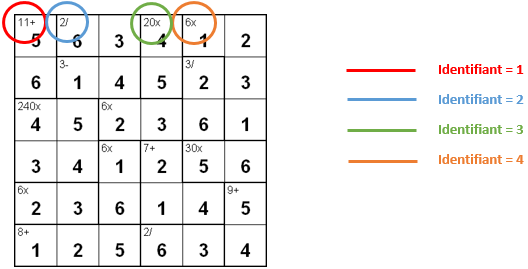
\includegraphics[scale=0.9]{identifiant_contrainte.PNG}
        \caption{Identifiant des contraintes}
    \end{figure}

    \section{Board}
    
Dans le vocabulaire que nous avons adopté, un board est une grille de KenKen en cours de remplissage. Ce terme est utilisé principalement dans la résolution pour désigner l'état de la grille qui en cours de résolution. De plus, dans la génération il représente la  solution de la grille en cours de remplissage.\par
Un board est constitué de chiffres en représentation décimale ou binaire (pour le solveur de logique) appelés Values.


\chapter{Besoins}

    \section{Fonctionnalités principales}
    
    Le logiciel doit avoir deux modes : \newline
    
    - la résolution de grilles \par
    - la génération de grilles \newline
    
    
    Il est lancé par la commande ./kenken
    
    > ./kenken -h \newline
    Usage: \newline
    kenken [-a|-o FILE|-v|-V|-h] FILE... \newline
    kenken -g[SIZE] [-u|-o FILE|-v|-V|-h] \newline
    Ce qui permet de résoudre ou générer des grilles KenKen de taille variable. \newline

    -g[N],--generate[=N] : génère une board de taille NxN (par défaut : 6x6)
    
    -a,--all : recherche toutes les solutions
    
    -u,--unique : génère une board n'ayant qu'une seule solution
    
    -o FILE,--output FILE : écrit les résultats dans un fichier FILE
    
    -v,--verbose : renseigne l'utilisateur sur les différentes étapes internes de la résolution ou de la génération des grilles.
    
    -V,--version : affiche la version du logiciel
    
    -h,--help : affiche l'aide utilisateur \newline

    Le logiciel s'interrompt en renvoyant un code \textit{EXIT\_FAILURE} en cas d'erreur.
    Sinon, il renvoie un code \textit{EXIT\_SUCCESS} dans le cas où tout s'est déroulé normalement.

    \section{Format d'entrée}
    
    Les fichiers donnés à l'analyseur suivent le format suivant.\newline
    
    \#blocs \newline
    \par
    \begin{tabular}{c c c c c c}
    1 & 2 & 2 & 3 & 4 & 4 \\
    1 & 5 & 5 & 3 & 6 & 4 \\
    7 & 7 & 8 & 8 & 6 & 4 \\
    7 & 7 & 9 & 10 & 11 & 11 \\
    12 & 12 & 9 & 10 & 10 & 13 \\
    14 & 14 & 14 & 15 & 15 & 13 \\ \newline
    \end{tabular} \newline
    
    \#Constraints \newline
    \par
    1: 11+ \par
    2: 2/ \par
    3: 20x \par
    4: 6x \par
    5: 3- \par
    6: 3/ \par
    7: 240x \par
    8: 6x \par
    9: 6x \par
    10: 7+ \par
    11: 30x \par
    12: 6x \par
    13: 9+ \par
    14: 8+ \par
    15: 2/ \\~\\
  
    - Les caractères espaces, tabulation, lignes vides et tout ce qui suit un '\#' (commentaire) sont ignorés. \newline

    - La grille doit être un carré de taille NxN (éventuellement définir une limite sur N).

    - Les caractères reconnus seront: '\#', '0-9', '1', ':', '+', '-', 'x', '/'.
    Tout autre caractère (en dehors d'un commentaire) provoque une erreur.

    - Les erreurs empêchant la lecture de la grille devront être dans le format suivant: \newline
    
    \textit{kenken: error: line 1: xxxxxxxxxxx} \newline

    Puis, le logiciel se termine en renvoyant un code EXIT\_FAILURE. \newline

    - Les avertissements signalent que le programme a pris une décision sur l'interprétation du fichier alors que plusieurs possibilités se présentaient à lui. Elles sont de la forme: \newline
    
    \textit{kenken: warning: line 1: xxxxxxxxxxx} \newline

    - Le parseur essaie toujours de comprendre le fichier et donne des messages d'erreur les plus compréhensibles possible. \newline


    \section{Format de sortie} 
    
    Le format de sortie des grilles résolues est le suivant: \newline

    > ./kenken ./example-grid.ken \newline
    
    Grid solved: \newline
    \begin{tabular}{c c c c c c}
    5 & 6 & 3 & 4 & 1 & 2 \\
    6 & 1 & 4 & 5 & 2 & 3 \\
    4 & 5 & 2 & 3 & 6 & 1 \\
    3 & 4 & 1 & 2 & 5 & 6 \\
    2 & 3 & 6 & 1 & 4 & 5 \\
    1 & 2 & 5 & 6 & 3 & 4 \\
    \end{tabular} \newline

            Le format de sortie des boards générées est le même que celui de l'entrée (cf au-dessus).

        \section{Standards et coding style}
            
            Le logiciel est programmé en C11 avec le coding style suivant: \newline

            Les commentaires, noms de variables, noms de fonctions sont en Anglais et suivent le standard suivant: \newline
            
            - \textit{function\_name\_example()} \newline
            - \textit{variable\_name\_example} \newline
            - \textit{typedef\_name\_example\_t} \newline

            - Une indentation du code est de 2 espaces de large.
            
            - Les tabulations sont mises à 8 espaces de large.
            
            - Les lignes ne dépassent pas les 80 colonnes.
            
            - Les commentaires sont toujours du type : /* ... */.
            
            - Nous mettons un espace autour des opérateurs binaires/ternaires, exemple: =  +  -  <  >  *  /  \%  |  \&  \^  <=  >=  ==  !=  ?  :
            
            - Nous mettons un espace après les opérateurs unaires, exemple: \&  *  +  -  ~  ! ++  --
            
            - Il n'y a pas d'espace autour des opérateurs de struct: '.' et '->'
            
            - Nous mettons un espace après les mots clés: 'if', 'switch', 'case', 'for', 'do', 'while'.
            
            - Nous avons choisi une manière consistante de placer les '{', '}'.
            
            - Toutes les macros sont en lettres capitales: \textit{\#define CONSTANT 0x12345}
            
            - Les commentaires sont ajoutés seulement lorsque c'est nécessaire.

        \section{Tests de couverture}
            
            Des grilles de tests avec une couverture de code d'au moins 90\% sont fournies.

        \section{Tests de charge et de profilage}
            
            Une analyse d'efficacité en profondeur est menée sur les différentes approches tentées.

        \section{Corpus de boards}
            
            Un corpus de grilles, classées par niveau de difficultés, doit être rendue à l'issue du projet, dont au moins une dizaine de grilles non-résolues par le logiciel (au moins une heure de calcul sans résultat).

        \section{Build-system}
            
            On utilise make pour construire le projet. Un Makefile est donc à la racine du projet et possède les règles suivantes: \newline

            \textit{make [all]}    Build all \newline
            \textit{make check}    Run coverage tests \newline
            \textit{make profile}  Run performance and load tests \newline
            \textit{make clean}    Remove all files generated by make \newline
            \textit{make help}     Display this help \newline
            
            La cible \textit{'all'} met le binaire \textit{'kenken'} à la racine. \newline

        \section{Structure du projet}
            
            kenken/
            
                \quad | \newline
                
                \quad +-Makefile \newline
                
                \quad +-doc/ \newline
                
                \quad +-include/ \newline
                
                \quad +-src/ \newline
                
                \quad +-test/

\chapter{Architecture et description du logiciel}


     KenKen2 est découpé en trois modules principaux : l'analyseur, le générateur et le solveur.

    \section{L'analyseur}

        L'analyseur (ou parser) parcours un fichier d'entrée et remplit une structure de données exploitable par les solveurs s'il est valide. Il suit les contraintes données par le client vues plus haut. Il n'est pas très robuste, beaucoup d'erreurs dans un fichier d'entrée mal rempli ne sont pas gérées. Cependant, tous les fichiers respectant le format d'entrée attendu sont traités correctement.

    \section{Le générateur}

        \begin{itemize}
            \item{\textbf{Module generator}} \newline

        Le module de génération de grilles Kenken se décompose en trois fonctions principales. La première est la génération de la boards. Au cours de son élaboration, notre projet Kenken connu trois versions différentes de la génération de boards. \newline
        
        La première version était très simple. Nous générions le board de haut en bas et de la gauche vers la droite. Ainsi case par case, l'algortihme générait un nombre aléatoire compris entre 1 et N. Il vérifiait si le nombre généré était présent dans les autres cases de la même colonne et de la même ligne. Si cela, n'était pas le cas, le nombre était introduit dans la case courante et l'algorithme passait à la case suivante, sinon il regénérait aléatoirement un nombre. \newline
        
        Cet algorithme était lent. Il produisait des grilles de taille 9x9 très difficilement. Une de nos premières optimisations fut de mémoriser à l'aide de deux matrices les nombres pouvant être générés dans chaque ligne et dans chaque colonne de la grille (\textit{Number-Ligne} et \textit{Number-Colonne}). Cela permettait d'éviter à l'algorithme de regénerer des nombres qu'il avait déjà utilisé plus tôt.
        L'algorithme allait plus vite et genérait des grilles de tailles plus grandes. \newline
        
        Cependant, generer des grilles de plus grande taille, mit en évidence un des défauts de cette méthode : un bug survenait quasiment systématiquement lorsque la taille de la grille excédait 10. Ce bug pouvait hypothétiquement arriver sur n'importe quelle grille de taille 3 ou plus. Néanmoins, si la taille de la grille restait basse, la probabilité pour qu'il apparaisse était très rare. Il fut donc difficile à discerner. \newline
        
        Pour le comprendre, nous allons simuler l'algorithme sur un cas d'utilisation. Admettons que l'utilisateur décide de generer une grille de taille 4. Tout se passe bien sur la première ligne de notre grille et nous obtenons pour l'instant le résultat suivant : \newline
        
        \end{itemize}

        \begin{figure}[h]
            \centering
                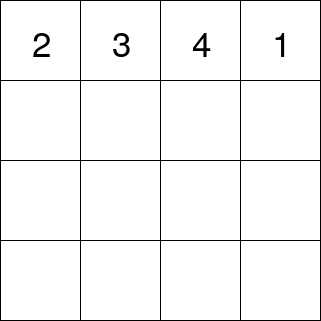
\includegraphics[scale=0.4]{2341.png}
        \end{figure}
        
        \newpage

        L'algorithme suit la même procédure et génère aléatoirement les trois cases de la ligne suivante: \newline

        \begin{figure}[h]
            \centering
                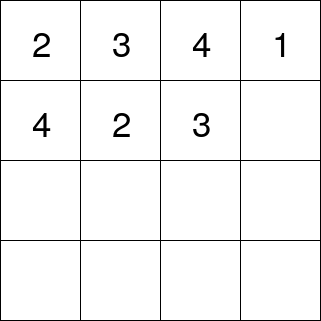
\includegraphics[scale=0.4]{423.png}
        \end{figure}

        Le programme s'enfermait alors dans une boucle infinie. Il ne parvenait pas à trouver de valeurs disponibles pour la dernière case de la ligne. Pour éviter cette boucle infinie, nous devions regenerer la ligne entière et par conséquent, remettre les matrices des disponibilités \textit{Number-Ligne} et \textit{Number-Colonne}, à jour. De plus rien ne permettait à l'algorithme d'éviter de regenerer une deuxième fois cette même séquence de nombres. \newline 
        
        Les performances de cet algorithme permettait de générer des grilles de taille 30x30. Néanmoins, au delà de 35*35, l'efficacité de l'algorithme était mise à l'épreuve. Il nous fallait donc un algorithme plus performant. \newline
        
        La deuxième version de la génération de grille était plus complexe. L'algorithme génerait la grille, ligne par ligne en tenant compte des disponibilités de chaque case de la ligne à generer. Pour nous aider à déterminer les disponibilités de chaque case, nous utilisions une matrice de boléens où les lignes de cette matrice représentaient les cases de la ligne en cours de génération et les colonnes représentaient les \textit{Numbers} disponibles. \newline
        
        Ainsi pour la grille G 3x3 ci dessous nous obtenions la matrice de disponibilités M suivantes pour les cases de la ligne 2: \newline
        
        \newpage
        
        \begin{figure}[h]
            \centering
                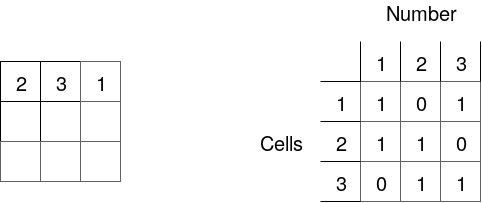
\includegraphics[scale=0.4]{disponibility1.PNG}
                \caption{Grille G (à gauche) avec sa matrice de disponibilité (à droite)}
        \end{figure}
     
        Avec cette matrice, l'algorithme déterminait d'abord la case avec le moins de \textit{Numbers} disponibles. S'il y en avait plusieurs, l'algorithme choisissait aléatoirement la case. L'algorithme choisissait ensuite parmi les \textit{Numbers} disponibles de cette case, le \textit{Number} étant le moins disponible pour toutes les cases de la ligne. Si on décide de générer la ligne suivante de cette matrice, l'algorithme itèrerait de la manière suivante : \newline
        
        \begin{itemize}
            \item{Etape 1.1} \newline

            Case 1 : 2 Numbers disponibles (1 et 3),
            
            Case 2 : 2 Numbers disponibles (1 et 2),
            
            Case 3 : 2 Numbers disponibles (2 et 3). \newline
            
            L'algorithme choisit donc aléatoirement une des cases. Par exemple la case 2. \newline

            \item{Etape 1.2} \newline

            Parmi les \textit{Numbers} disponible de la case 2 :
            
            Number 1 : disponible 2 fois (dans la case 1 et la case 2),
            
            Number 2 : disponible 2 fois (dans la case 2 et la case 3),
            
            L'algorithme choisit donc aléatoirement un des \textit{Numbers} de la case 2, prenons par exemple le 1. Nous avons donc la matrice G et la matrice de disponibilité suivante : \newline
            
            \newpage

            \begin{figure}[H]
                \centering
                    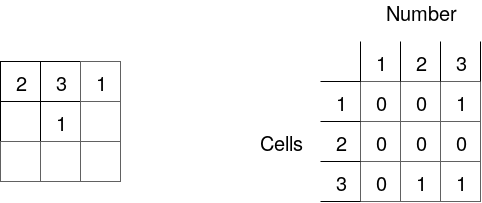
\includegraphics[scale=0.4]{disponibility2.PNG}
                    \caption{Grille G (à gauche) avec sa matrice de disponibilité (à droite)}
            \end{figure}
        
            \item{Etape 2.1} \newline

            case 1 : 1 Numbers disponibles (le 3),
            
            case 3 : 2 Numbers disponibles (2 et 3). \newline
            
            La case 1 a moins de \textit{Numbers} disponibles que la case 3. L'algorithme choisit donc la case 1. \newline

            \item{Etape 2.2} \newline

            Seul le \textit{Number} 3 est disponible dans la case 1. Nous avons donc la matrice G et la matrice de disponibilité suivante: \newline

            \begin{figure}[H]
                \centering
                    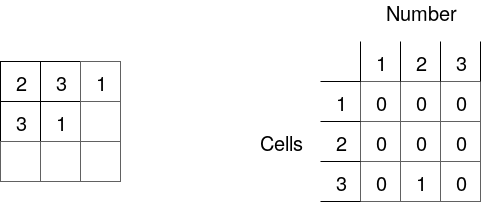
\includegraphics[scale=0.4]{disponibility3.PNG}
                    \caption{Grille G (à gauche) avec sa matrice de disponibilité (à droite)}
            \end{figure}

            \item{Etape 3} \newline

            Il ne reste qu'une seule case avec un seul \textit{Number} disponible. On complète donc la ligne courante avec le \textit{Number} 2 en case 3. \newline

            Les performances de cet algorithme étaient nettement meilleures que celles de la première version. L'algorithme générait des grilles de taille 100x100 en moins d'une seconde et des grilles de 200*200 en moins de 10 secondes. \newline 
            
            Cependant, comme la première version de notre algorithme, celle ci pouvait génerer une ligne bloquante au cours de la génération et bloquer le programme dans une boucle infinie. Il fallait donc, comme la première version de l'algorithme, réinitialiser la ligne en cours de génération et la matrice des disponibilités \textit{Case-Number}. \newline
            
            Là aussi, rien n'empêchait notre algorithme de regénerer cette même ligne. Il nous fallait donc réfléchir à un troisième algorithme ne pouvant hypothétiquement pas se bloquer. \newline

            Pour parer ce problème, la troisième version de notre algorithme utilise la propriété suivante qui s'applique aux carrés latins : \newline 
            
            \textbf{Interchanger deux lignes ou deux colonnes dans un carré latin n'affecte pas les propriétés de celui-ci.} \newline
            
            Lorsque l'utilisateur choisit de générer une grille, l'algorithme commence toujours par créer le même carré latin. Seule la taille de celui ci varie. L'algorithme est ensuite amené à interchanger les lignes et les colonnes aléatoirement un certain nombre de fois. Le nombre de modifications effectuées est déterminé en fonction de la taille de la grille à generer. \newline
            
            En plus d'être beaucoup plus simple que la version précedente, cet algorithme ne risque hypothétiquement pas de créer une structure bloquante au cours de la géneration. Il n'y a donc pas de verifications, ni de "marches arrières" dans cet algorithme qui ralentissaient les performances des deux autres. \newline
            
            Cet algorithme génère des grilles de 300*300 en 2 secondes, des grilles de 500*500 en 30 secondes et des grilles 1000*1000 en 20 minutes. \newline

            La deuxième fonction de génération est la géneration des blocs. Le mécanisme de génération se fait de haut en bas et de la gauche vers la droite et suit la procédure suivante : \newline
            
            L'algorithme cherche d'abord une case C sans identifiant de contrainte. Il détermine ensuite une taille aléatoire T pour le bloc qu'il va dessiner. Cette taille est déterminée en fonction de la taille minimum et de la taille maximum de bloc que l'algorithme reçoit de l'utilisateur. \newline 
            
            À partir de ces données, l'algorithme choisit parmi les directions disponibles à partir de la
            case C. Une direction est disponible si, à partir de la case C, on ne va ni vers une case possédant déjà un identifiant de contrainte, ni au delà d'un bord de la grille. \newline 
            
            Si une direction est disponible, l'algorithme va changer l'identifiant de contrainte de la case voisine qui se trouve dans cette direction et la prendre comme case courante. \newline 
            
            L'algorithme répète cette action T fois ou jusqu'à ce qu'il tombe sur une case qui n'a aucune direction disponible pour former un bloc. La procédure est terminée lorsque la grille ne possède plus de case qui n'appartienne à aucun bloc. \newline
            
            Le problème de cette méthode est qu'il ne permet pas de générer certains types de blocs qui sont pourtant possibles dans toutes les grilles de Kenken. Pour cette raison nous avons envisagé une amélioration de l'algorithme décrit ci dessus. \newline
            
            Au lieu de sélectionner la case récemment ajoutée au bloc comme case courante, l'algorithme peut sélectionner aléatoirement une case parmi toutes les cases du bloc que l'algorithme est en train de dessiner. Il faut pour cela, ajouter un tampon qui permet à l'algorithme de mémoriser les cases qu'il vient d'ajouter au bloc. Nous nous sommes également interessés aux algorithmes de pavage avec générations aléatoires de polyominos sans pour autant avoir l'occasion d'en implémenter un. \newline

            La troisième fonction de génération est la génération des contraintes de bloc. Pour cela, notre algorithme va chercher dans notre grille de blocs,  les cases appartenant à chacun de nos blocs et placer leur Value dans un tampon. \newline
            
            L'algorithme choisit ensuite aléatoirement un opérateur si le bloc contient plus d'une case. Si l'opérateur ne convient pas (division non entière, différence négative, multiplication ou addition dépassant la limite du type \textit{int} dans le langage C), un nouvel opérateur est choisi aléatoirement. \newline


        \end{itemize}

\chapter{Les solveurs}

\section{Solveur par backtracking}

L'algorithme de backtracking est un algorithme de recherche de solution. Il explore toutes les solutions d'un problème naïvement jusqu'à en trouver une. Voici la façon dont il procède pour une grille de KenKen de dimension N :\\

\begin{algorithm}
\caption{Recursive backtracking}
\begin{algorithmic}[1]
\STATE integer i, j
\STATE Find an empty case on the board, store its coordinates in i,j
\IF {such a case exists}
\FOR {$n \gets 1 : N$}
\IF {n in case i,j is a valid move}
\STATE Insert n in i, j
\IF {Recursive backtracking}
\STATE Return true
\ELSE
\STATE Reset case i,j to 0 
\ENDIF
\ENDIF
\ENDFOR
\STATE Return false
\ELSE
\STATE Return true
\ENDIF

\end{algorithmic}
\end{algorithm}

Cet algorithme ne fait que remplir les cases du board séquentiellement jusqu'à trouver une combinaison valide. Sa complexité est dans le pire des cas en \textit{$O(N^{N^2})$}. Cette complexité le rend impraticable sur des grilles de grande taille.

\section{Solveur de système de contraintes : Z3}

    Le Module de résolution à l'aide du solveur Z3 contient des fonctions permettant d'exprimer une grille de Kenken sous la forme d'un système de contraintes. Le projet Kenken2 comprend trois méthodes différentes de résolutions. Chacune de ces méthodes se différencie par la manière d'exprimer le système à résoudre par le solveur Z3. Afin d'apporter une meilleure compréhension à cette partie du projet Kenken2, nous allons d'abord apporter les définitions à chaque terme employé : \newline
    
    - Une \textit{expression} est une équation ou une inéquation.
    
    - Un \textit{système} est un ensemble d'\textit{expression}.
    
    - Un \textit{terme} est un des deux côtés de l'\textit{expression}.
    
    - Un \textit{argument} est un des éléments d'un \textit{terme}. \newline

    Donc pour ce \textit{système}: \newline

    (1) x + 2y + z = a - c
    
    (2) 2a - b > 3 \newline

    x + 2y + z = a - c est une \textit{expression}.
    
    b > 2a + z est une \textit{expression}.
    
    x + 2y + z est le \textit{terme} gauche de l'\textit{expression} (1).
    
    a - c est le \textit{terme} droit de l'\textit{expression} (1).
    
    2a est un \textit{argument} du \textit{terme} gauche de l'\textit{expression} (2).
    
    3 est l'\textit{argument} du \textit{terme} droit de l'\textit{expression} (2) et le \textit{terme} droit de
    l'\textit{expression} (2). \newline

    Pour exprimer une grille de Kenken sous la forme d'un système de contraintes, nous allons d'abord étudier les différents types de contraintes qu'une grille de Kenken possède : \newline
    
    - La solution d'une grille de Kenken est un carré latin.
    
    - Une grille de Kenken est entièrement parcouru par des blocs. \newline
    
    Pour exprimer ces contraintes sous la forme d'(in)équations, nous allons attribuer une variable pour chaque case de notre grille. 
    
    Ainsi pour la grille G 3x3 ci-dessous, nous obtenons les variables suivantes: \newline

    \begin{tabular}{| c | c | c |}
        \hline
        x0 & x1 & x2 \\ \hline
        x3 & x4 & x5 \\ \hline
        x6 & x7 & x8 \\
        \hline 
    \end{tabular} \newline
    
    Pour un carré latin de taille n, les contraintes sont les suivantes: \newline
    
    - Chaque ligne contient en un seul exemplaire des n éléments distincts de l'intervalle composé des entiers de 1 à n.
    
    - Chaque colonne contient en un seul exemplaire les n éléments distincts de l'intervalle composé des entiers de 1 à n.
    
    - Chaque case contient un chiffre appartenant à l'intervalle composé des entiers de 1 à n. \newline

    Nous avons trouvé deux manières différentes d'exprimer ces trois principes. \newline
    
    \begin{itemize}
        \item{Première approche} \newline
        
        Exprimer le système de contraintes sous forme d'inéquations linéaires. On obtiendrait donc : \newline
        
        - Chaque case est différente de toutes cases qui partagent la même ligne et la même colonne que cette dernière.
        
        - La valeur de chaque case est supérieure strictement à 0 et inférieur à \newline n + 1. \newline

        Pour la case x0 de la board G de dimension 3x3 ci dessus, nous obtenons les premières inéquations suivantes: \newline
        
        x0 != x1, 
        
        x0 != x2, 
        
        x0 != x3, 
        
        x0 != x6, 
        
        x0 > 0 
        
        et x0 < 4. \newline
        
        \item{Deuxième approche} \newline
    
        La seconde manière d'exprimer ce système de contraintes est de le faire sous la forme d'équations non-linéaires. Nous choisissons d'exprimer chaque ligne et chaque colonne sous la forme d'une somme et d'un produit rendant ainsi leur décomposition unique. \newline
        
        Le but de cette représentation est de produire moins de contraintes dans notre système et donc de rendre sa résolution potentiellement plus rapide. Pour la première ligne de notre grille G de
        dimension 3x3 ci dessus, nous obtenons seulement ces 2 contraintes: \newline
        
        x0 + x1 + x2 = 6 
        
        et x0 * x1 * x2 = 10. \newline

        On passe ainsi d'un système avec \newline 2 + TRIANGLE\_DE\_PASCAL(dimension\_de\_la\_board - 1) contraintes par lignes et par colonnes à un système avec 2 contraintes par lignes et par colonnes.
        
        Cependant, l'une de ces deux contraintes est alors exprimée sous la forme d'une équation non-linéaire. Malgré la réduction du nombre de contraintes permise par cette représentation, la résolution de ce type de contrainte est très complexe. Cela rend donc la résolution beaucoup plus fastidieuse que la représentation sous forme d'inéquations linéaires. \newline

        Les solveurs nommés \textit{inequalities\_system} et \textit{linear\_inequalities\_system} utilisent la première méthode pour exprimer les contraintes du carré latin.
        
        Le solveur nommé \textit{equations\_system} utilise la seconde méthode pour exprimer les contraintes du carré latin. \newline

        Les blocs de nos grilles de Kenken s'expriment de deux manières différentes.
        
        D'un côté nous distinguons les égalités (si notre bloc ne contient qu'une seule case), les sommes et les différences. Ces contraintes sont exprimées de la même manière dans les deux représentations que nous avons mis en place.
        
        Et d'un autre côté nous distinguons les multiplications et les divisons qui peuvent être représentées linéairement ou non. \newline

        Pour la grille G de dimension 3x3 nous conservons les mêmes variables que celles attribuées plus haut. Nous lui ajoutons cependant une représentation par blocs avec les contraintes qui les accompagnent: \newline

        \begin{figure}[H]
            \centering
            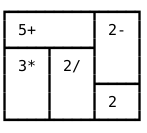
\includegraphics[scale=0.9]{kenekn3.png}
        \end{figure}

        Ayant un résultat bien précis, les blocs sont donc tous représentés sous la forme d'équations. Dans le cas des égalités, l'algorithme place l'unique case appartenant à ce bloc comme \textit{terme} gauche de notre équation et le résultat comme \textit{terme} droit. \newline

        Dans le cas d'une somme, l'algorithme applique une somme entre toutes les cases du bloc courant. Il place ce résultat comme \textit{terme} gauche de notre équation et le résultat comme \textit{terme} droit. \newline

        Dans le cas d'une différence, l'ordre des arguments du \textit{terme} gauche de notre equation est primordial pour trouver le résultat du \textit{terme} droit.
        
        Malheureusement, l'algorithme ne peut savoir laquelle des cases du bloc a la valeur la plus haute. Notre algorithme effectue donc une première soustraction entre les cases du bloc. Il place ce résultat comme \textit{terme} gauche de notre première équation et le résultat comme \textit{terme} droit. \newline
        
        L'algorithme stocke ensuite cette equation dans un tampon d'\textit{argument} pour notre \textit{expression} finale. L'algortihme substitue le premier \textit{argument} de notre première soustraction avec son deuxième \textit{argument}. 
        
        À partir de ceci, il construit une nouvelle équation qu'il stocke là aussi dans son tampon. L'algorithme réalise ce traitement autant de fois qu'il y a de cases dans le bloc. \newline
        
        L'algorithme finit par effectuer un OR sur chaque élément du tampon d'\textit{arguments} qu'il a construit. \newline

        Dans le cas de la représentation non-linéaire des blocs dont la contrainte opérationnelle est une multiplication, l'algorithme applique un produit comme \textit{terme} gauche de notre équation et le résultat comme \textit{terme} droit. 
        
        La division, quant a elle, est semblable au traitement réalisé en cas de soustraction. La seule différence est qu'il aura un tampon dont les \textit{arguments} sont des équations dont les \textit{termes} gauches sont des divisions. Pour les blocs de notre grille G, la première représentation sous forme de système d'\textit{expression} est la suivante : \newline

        (1) x0 + x1 = 5
        
        (2) (x2 - x5 = 2) | (x5 - x2 = 2)
        
        (3) x3 * x6 = 3
        
        (4) (x4 / x7 = 2) | (x7 / x4 = 2)
        
        (5) x8 = 2 \newline

        Dans le cas de la représentation linéaire des blocs dont la contrainte opérationnelle est une multiplication ou une division, l'algorithme effectue un même traitement qui est le suivant. 
        
        Il va d'abord chercher les combinaisons avec répétition de longueur égale aux nombre de cases dans le bloc et dont les objets sont compris dans l'ensemble des entiers de 1 à n (n étant la dimension de la
        board). 
        
        Pour chacune des combinaisons avec répétition, l'algorithme effectue une multiplication (ou une division selon la contrainte opérationnelle du bloc) dont chaque \textit{argument} est un objet de cette
        combinaison. 
        
        Si le résultat de cette opération est égal au résultat de la contrainte du bloc, alors notre algorithme stocke une équation dont le \textit{terme} droit est la somme de ces objets et le \textit{terme} gauche est la somme des cases du bloc. \newline
        
        L'algorithme termine en effectuant un OR sur chaque élément de son tampon. Pour les blocs de notre grille G, on obtient cette seconde représentation : \newline

        (1) x0 + x1 = 5
        
        (2) (x2 - x5 = 2) | (x5 - x2 = 2)
        
        (3) x3 + x6 = 4
        
        (4) x4 + x7 = 3
        
        (5) x8 = 2 \newline

        L'avantage de cette représentation sur la première est qu'elle évite d'encombrer notre système avec des \textit{expressions }non-linéaires. 
        
        Cela permet donc au solveur Z3 de résoudre plus rapidement notre \textit{système} d'\textit{expression}. \newline
        
        Le problème que pose cette représentation est le suivant : ce traitement affaiblit la contrainte initiale. L'\textit{expression} linéarisée proposée par notre représentation n'est pas la même que celle que le bloc exprime. 
        
        L'algorithme est donc contraint d'effectuer une vérification après coup sur la solution proposée par
        le solveur Z3. 
        
        Si la solution proposée par le solveur Z3 ne vérifie pas les contraintes exprimées initialement par les blocs de notre grille, alors notre algorithme ajoute une contrainte au système pour signifier à Z3 que la solution qu'il vient de trouver n'est pas celle attendue par l'utilisateur. \newline

        Les solveurs nommés \textit{equations\_system} et \textit{inequalities\_system} utilisent la
        première méthode pour exprimer les contraintes des blocs. 
        
        Le solveur nommé \textit{linear\_inequalities\_system} utilise la seconde méthode pour exprimer les
        contraintes des blocs de la grille. \newline

        En terme de performance, le solveur \textit{equations\_system} est le moins efficace. 
        
        Qu'il s'agisse des contraintes du carré latin ou des contraintes des blocs, il emploie leurs représentations non linéaires. 
        
        La taille de grille qu'il peut résoudre ne dépasse pas 4x4, avec une baisse de performance si la grille contient des blocs dont la contrainte opérationnelle est une multiplication ou une division. \newline
        
        Le solveur \textit{inequalities\_system} parvient à résoudre des grilles 6x6. 
        
        Cependant la même baisse de performance est observée si les blocs contiennent des multiplications ou des divisions. En sachant qu'il représente les contraintes du carré latin de la grille sous forme linéaire, il est normal d'observer une meilleure efficacité. \newline
        
        Le meilleur solveur est donc logiquement \textit{linear\_inequalities\_system}. 
        
        Avec ce solveur, toutes les contraintes de la grille sont représentées sous forme linéaire. Il résoud des grilles de taille 9x9 avec 10 secondes de moyenne. Cette durée peut s'allonger à de rares occasions jusqu'à 30 secondes.
    
    \end{itemize}

\section{Solveur logique}

Le jeu KenKen étant un dérivé du Sudoku, il est naturel de penser à une approche logique pour résoudre une grille. On représente alors la grille par un tableau d'ensemble de possibilités, correspondant aux chiffres possibles dans les cases de la grille. L'algorithme de résolution logique se construit sur celui de backtracking, à la différence qu'il applique des principes de logique sur ces ensembles. Cette approche plus "humaine" augmente grandement les performances pour cette raison.\par
Chaque case de la grille comporte N bits, le i-ème bit représentant la possibilité que i soit dans la case. Si le bit est à 1, le chiffre est possible, 0 sinon. Au début du programme, tous les bits sont à 1. L'objectif est de ne trouver le m\^eme bit qu'une seule fois par ligne et colonne, et que chaque case n'ait plus qu'un bit à 1.

\begin{algorithm}[H]
\caption{Logic}
\begin{algorithmic}[1]
\WHILE {The grid has been modified}
\STATE Apply the logic rules on the board
\ENDWHILE

\IF{The grid is not solved}
\STATE integer i, j
\STATE Find an empty case on the board, store its coordinates in i,j
\IF {Such a case exists}
\STATE Make a copy of the current board
\FOR {$n \gets 1 : N$}
\IF {n in case i,j is a possible move}
\STATE Set all bits but the n-th in i, j to 0 in the copy
\IF {Logic on the copy}
\STATE Return true
\ELSE
\STATE Reset the copy to the current board
\ENDIF
\ENDIF
\ENDFOR
\ENDIF
\STATE Return false
\ENDIF
\STATE Return true

\end{algorithmic}
\end{algorithm}

Tout l'intérêt de cette approche est de trouver des règles logiques efficaces pour éliminer le plus de possibilités.

\subsection{Règles de contrainte}

La première logique appliquée est casee du respect des règles de contrainte. Les chiffres présents dans une bloc doivent en effet, combinés avec l'opérateur correspondant, arriver exactement à la cible de la bloc. La méthode "update\_blocs" parcours donc tous les blocs, et pour chacun calcule la somme, la multiplication, la division ou la soustraction de toutes les possibilités de chaque case du bloc. De ces calculs, il ne garde que les possibilités qui ont été utilisées pour arriver au bon résultat, et met à 0 casees qui n'ont jamais été dans un calcul concluant.\par
Voici un exemple de passage par "update\_rooms" pour un bloc de taille 2 et de contrainte 4+ :

\begin{figure}[H]
\centering
   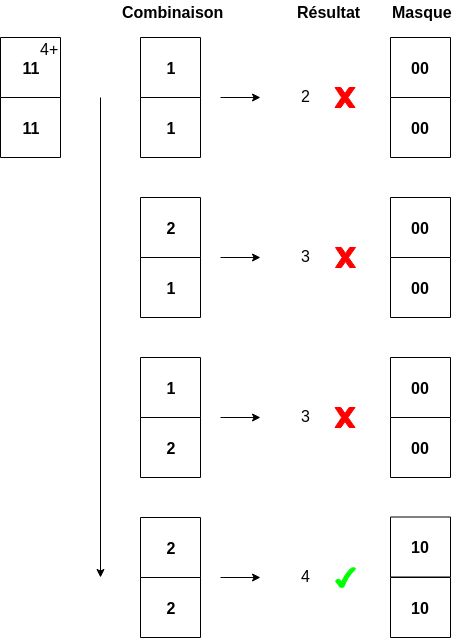
\includegraphics[scale=0.45]{update_rooms_changes.png}
   \caption{Principe des masques de update\_blocs}
\end{figure}

Les deux cases du bloc ont leur deux premiers bits à 1, ce qui laisse donc la possibilité à 1 et 2 d'être dans ces cases. Afin de savoir quels chiffres vont mener à une somme égale à 4, on se munit de masques de 2 bits qui stockeront cette information. Pour cela, on intialise un masque à 0 par case du bloc, et pour chaque combinaison amenant à 4, on mettra le bit correspondant à 1. Ainsi, aux trois premières tentatives, la somme n'arrive pas à 4 et les bits des masques ne sont pas mis à jour. Puis la dernière combinaison fonctionne, un 2 dans les deux cases, et les deuxième bits des masques sont mis à 1.\par
Lorsque toutes les combinaisons sont vues, les masques sont appliqués sur les cases correspondantes. De cette façon, uniquement les possibilités amenant effectivement à la solution sont conservées.


\section{Règle du carré latin}

Cette règle vérifie qu'un nombre ne peut être présent qu'une fois par ligne et par colonne.\par
Elle est implémentée par la méthode "update\_rows\_cols" qui dès qu'une case n'a qu'une possibilité, retire cette possibilité des autres cases de sa ligne et colonne.

\subsection{Règle du naked subset}

Le principe du naked subset est le suivant : Si on peut trouver dans une m\^eme ligne (resp. colonne) X possibilités et exactement X cases composées uniquement de ces possibilités, alors ces X possibilités peuvent être retirées de toutes les autres cases de la ligne (resp. colonne).

\begin{figure}[H]
\centering
   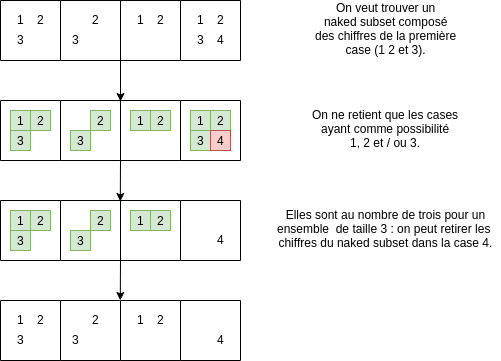
\includegraphics[scale=0.45]{naked_subset.png}
   \caption{Principe du naked subset sur une ligne de taille 4}
\end{figure}

Pour implémenter cette règle, l'algorithme parcours chaque case, et vérifie si son ensemble de possibilité constitue un naked subset dans sa ligne ou sa colonne.\par
La complexité de notre implémentation est en \textit{O}($N^3$). Une piste pour l'améliorer serait de ne pas essayer de trouver de naked subset passé une taille d'ensemble arbitraire, mais n'ayant pas de tests permettant de déterminer cette taille nous avons opté pour une approche exhaustive.


\subsection{Règle du hidden subset}

Le principe du hidden subset est le suivant : Si on peut trouver X possibilités partagées exclusivement par X cases d'une m\^eme ligne (resp. colonne), alors on peut exclure toutes les autres possibilités de ces cases.

\begin{figure}[H]
\centering
   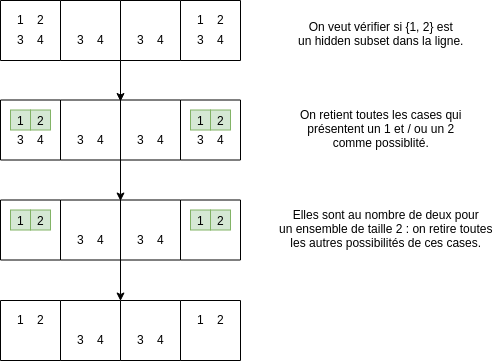
\includegraphics[scale=0.45]{hidden_subset.png}
   \caption{Principe du hidden subset sur une ligne de taille 4}
\end{figure}

Notre implémentation ne vérifie que l'existence de hidden subset de taille 2. Une amélioration évidente serait de le faire jusqu'à une taille arbitraire, mais la difficulté pour cela est de trouver une façon efficace de faire varier la taille de cet ensemble.\par

\chapter{Réalisations annexes}

    La recherche de solveurs performants nous a amené à des solutions intéressantes que nous n'avons pas pu tester, mais qu'il nous semblait judicieux de ne pas laisser de c\^oté. \newline
    
    Du problème Kenken au problème de couverture exacte : \newline
    
    Le problème Kenken, de la même manière que le problème Sudoku, peut vraissemblablement se réduire à celui de couverture exacte. 
    
    Le problème de couverture exacte est de trouver une couverture exacte pour un ensemble U et une collection S de sous-ensembles de U. On peut représenter une instance du problème de couverture exacte par un graphe biparti où d'un côté on retrouve notre collection S et de l'autre on a notre ensemble U. \newline
    
    Si un sous-ensemble appartenant à S contient un élément de l'ensemble U alors une arrête relie les deux sommets qui les représentent. La couverture exacte est donc un ensemble de sommets S' représentant des sous-ensembles dans S de telle manière qu'il existe une unique arrête entre un sommet de S' et chaque sommet dans U. \newline
    
    \begin{figure}[h]
    \centering
        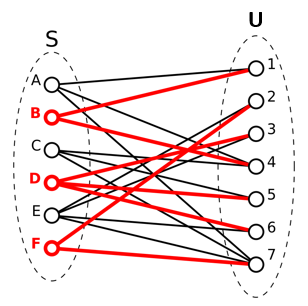
\includegraphics[scale=0.9]{couvertureexacte.PNG}
        \caption{Couverture exacte représentée sous la forme d'un graphe biparti}
    \end{figure}
    
    
    
    Avant d'entamer une réduction commençons par énoncer les contraintes posées par une grille Kenken de taille n: \newline
    
    - Chaque case doit contenir un nombre entre 1 et n.
    
    - Chaque ligne et chaque colonne doit contenir chacun des nombres compris entre 1 et n exactement une fois.
    
    - Toutes les contraintes des blocs doivent être satisfaites. \newline
    
	Chaque assignation possible d'un Number à une case sera représentée en suivant la convention suivante:
	
	L pour Ligne, C pour Colonne et N pour Number. 
	
	Donc la possibilité d'attribuer le Number 1 à la première case (donc la case de la Ligne 1 et de la Colonne 1) est notée ainsi: L1C1N1. \newline
	
    Pour représenter notre grille Kenken sous la forme  d'un problème d'ensemble intersectant exact, nous allons procéder à la réduction vers Exact Cover de manière méthodique. Nous commençons d'abord par reduire les contraintes du carré latin puis les contraintes des blocs du problème Kenken à des éléments de l'ensemble U dans le problème Exact Cover. Nous allons illustrer cette réduction sur la grille G de taille 3*3 ci-dessous: \newline

    \begin{figure}[h]
        \centering
            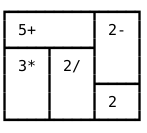
\includegraphics[scale=0.9]{kenekn3.png}
            \caption{Grille G}
    \end{figure}
    
    Les contraintes d'une grille Kenken peuvent être représentées par des ensembles de contraintes. Pour les contraintes du carré latin nous pouvons répartir les contraintes entre trois ensembles différents: \newline
    
    - Un ensemble de contraintes Ligne-Colonne contient toutes les possibilités pour une case. Par exemple pour l'ensemble des contraintes de la première case (c'est à dire celle de la ligne 1 et de la colonne 1) contient les possibilités suivantes:
    
    L1C1 = {L1C1N1, L1C1N2, L1C1N3} \newline
    
    - Un ensemble de contraintes Ligne-Number contient toutes les possibilités pour une ligne particulière et la place de ce Number à l'interieur. Par exemple pour l'ensemble des contraintes pour la ligne 1 et le Number 1, cela donne l'ensemble suivant:
    
    L1N1 = {L1C1N1, L1C2N1, L1C3N1} \newline
    
    - Un ensemble de contraintes Colonne-Number contient toutes les possibilités pour une colonne particulière et la place de ce Number à l'interieur. par exemple pour l'ensemble des contraintes pour la colonne 1 et le Number 1, nous obtenons l'ensemble suivant:
    
    C1N1 = {L1C1N1, L2C1N1, L3C1N1} \newline
    
    Pour les contraintes de blocs, en plus de conserver les étiquettes attribuées aux lignes, colonnes et Numbers, nous adoptons une convention supplémentaire pour représenter ce que notre notation actuelle ne nous permet pas d'exprimer. Une contrainte dans le problème Kenken réduite au problème de couverture exacte est notée de la manière suivante : \newline
    
    (\{Cible\}\{Operateur\}\{(case(s))\}) \newline
    
    Nous avons donc un nouvel ensemble de contraintes qui contient, pour une contrainte, toutes les possibilités de permutations avec répétitions qui satisfont la contrainte. Par exemple, pour l'ensemble des contraintes de la contrainte 5+ de notre grille G, nous obtenons : \newline
    
    5+(L1C1)(L1C2) = \{5+(L1C1N2)(L1C2N3), 5+(L1C1N3)(L1C2N2)\} \newline
    
    Pour la grille G ci dessus cela nous donne donc l'ensemble U suivant: \newline
    
    - Les ensembles Ligne-Colonne: \newline
    
    L1C1 = \{L1C1N1, L1C1N2, L1C1N3\},
    
    L1C2 = \{L1C2N1, L1C2N2, L1C2N3\},
    
    L1C3 = \{L1C3N1, L1C3N2, L1C3N3\},
    
    L2C1 = \{L2C1N1, L2C1N2, L2C1N3\},
    
    L2C2 = \{L2C2N1, L2C2N2, L2C2N3\},
    
    L2C3 = \{L2C3N1, L2C3N2, L2C3N3\},
    
    L3C1 = \{L3C1N1, L3C1N2, L3C1N3\},
    
    L3C2 = \{L3C2N1, L3C2N2, L3C2N3\},
    
    L3C3 = \{L3C3N1, L3C3N2, L3C3N3\} \newline
    
    - Les ensembles Ligne-Number: \newline
    
    L1N1 = \{L1C1N1, L1C2N1, L1C3N1\},
    
    L1N2 = \{L1C1N2, L1C2N2, L1C3N2\},
    
    L1N3 = \{L1C1N3, L1C2N3, L1C3N3\},
    
    L2N1 = \{L2C1N1, L2C2N1, L2C3N1\},
    
    L2N2 = \{L2C1N2, L2C2N2, L2C3N2\},
    
    L2N3 = \{L2C1N3, L2C2N3, L2C3N3\},
    
    L3N1 = \{L3C1N1, L3C2N1, L3C3N1\},
    
    L3N2 = \{L3C1N2, L3C2N2, L3C3N2\},
    
    L3N3 = \{L3C1N3, L3C2N3, L3C3N3\} \newline
    
    - Les ensembles Colonne-Number: \newline
    
    C1N1 = \{L1C1N1, L2C1N1, L3C1N1\},
    
    C1N2 = \{L1C1N2, L2C1N2, L3C1N2\},
    
    C1N3 = \{L1C1N3, L2C1N3, L3C1N3\},
    
    C2N1 = \{L1C2N1, L2C2N1, L3C2N1\},
    
    C2N2 = \{L1C2N2, L2C2N2, L3C2N2\},
    
    C2N3 = \{L1C2N3, L2C2N3, L3C2N3\},
    
    C3N1 = \{L1C3N1, L2C3N1, L3C3N1\},
    
    C3N2 = \{L1C3N2, L2C3N2, L3C3N2\},
    
    C3N3 = \{L1C3N3, L2C3N3, L3C3N3\} \newline
    
    - Les ensembles Bloc: \newline
    
    5+(L1C1)(L1C2) = \{5+(L1C1N2)(L1C2N3), 5+(L1C1N3)(L1C2N2)\},
    
    2-(L1C3)(L2C3) = \{2-(L1C3N1)(L2C3N3), 2-(L1C3N3)(L2C3N1)\},
    
    3*(L2C1)(L3C1) = \{3*(L2C1N1)(L3C1N3), 3*(L2C1N3)(L3C1N1)\},
    
    2/(L2C2)(L3C2) = \{2/(L2C2N1)(L3C2N2), 2/(L2C2N2)(L3C2N1)\},
    
    2=(L3C3) = \{L3C3N2\} \newline
    
    Maintenant que nous sommes capable de réduire une grille de Kenken vers une instance du problème de Couverture Exacte, il ne nous reste plus qu'à appliquer un algorithme qui permet de trouver des solutions au problème de Couverture Exacte. L'algortihme X de Knuth permet de résoudre des solutions à ce problème si l'instance du problème est représentée sous la forme d'une matrice booléenne. \newline
    
    De façon générale, pour chaque case d'une grille Kenken de taille n, il sera assigné un Number. Ajoutons à cela, les possibilités engendrées par la réduction des contraintes. Leur nombre est difficilement prévisible puisqu'il est dépendant de la taille de la grille Kenken, de la taille de la contrainte et de l'opérateur de la contrainte. Appelons ce nombre e. \newline
    
    On peut donc affirmer que la réduction vers Couverture Exacte engendre la création d'une collection S de ($n^{3}$ + e) possibilités. Le nombre d'ensemble de contraintes est plus facilement quantifiable. Pour les ensembles Ligne-Colonne, il en existe n*n, pour les ensemble Ligne-Number, il en existe n*n, pour les ensembles Colonne-Number, il en existe n*n et pour les ensembles Bloc, il en existe autant qu'il y a de contraintes (appelons ce nombre m). \newline
    
    La réduction vers Couverture Exacte engendre la création d'un ensemble U de taille 3*m*n. Pour une grille Kenken, l'algorithme X de Knuth manipule une matrice booléenne dont la taille sera de ($n^{3}$ + e) * (3*m*n). \newline
    
    Notre matrice booléenne est composée en ligne, des sous-ensemble de U présents dans notre collection S, et en colonne, des éléments de U. Si un élément de U est présent dans un sous ensemble de notre collection S alors la valeur \textit{TRUE} sera entrée pour la case correspondante de la matrice booléenne. \newline
    
    Pour la grille G au dessus, nous aurions une matrice de taille assez conséquente, elle est donc trop difficile à représenter. \newline
    
    Il ne nous resterait donc plus qu'à appliquer l'algorithme X de Knuth : \newline
    
    Algorithme X de Knuth:
    \begin{algorithm}[H]
\caption{Logic}
\begin{algorithmic}[1]

    
    Boolean matrix M;
    \WHILE (M is not empty) DO:
    	Determine the colomn C which contains the least of TRUE in M;
        Choose a row L such M[L][C] == TRUE;
        Add L in the partial solution;
        \FOR (column J such M[L][J] == TRUE) DO:
            \FOR (row I such M[I][J] == TRUE) DO:
                Delete I from M;
            \ENDFOR
            Delete J from A;
        \ENDFOR
    \ENDWHILE
    
    

\end{algorithmic}
\end{algorithm}

\chapter{Compte rendu exhaustif des séances de TD}

    \section{TD \#1 du 24/01/2019 : "Première version du document d'analyse des besoins, bibliographie, compréhension du domaine et ébauche des objectifs de première release".}

        \begin{itemize}

            \item \textbf{Première version du document d'analyse des besoins}

            De nombreuses remarques ont été faites sur notre première version du cahier des besoins. Tout d'abord, il nous a été rappelé de spécifier un degré de priorité sur \textbf{toutes} les options prises en compte par notre exécutable.
            Nous avions placé l'explication de l'option \emph{-v}, \emph{--verbose}, dans la partie des besoins fonctionnels, ce qui était une erreur, nous devions donc la placer dans la partie des besoins non-fonctionnels.

            En ce qui concerne les besoins non-fonctionnels, Mr. Archipoff nous a évoqué d'y préciser le besoin de quantification, c'est à dire réussir à avoir des temps de référence, savoir si tel algorithme de résolution est meilleur sur telle grille. Nous devions aussi parler du profiling, des tests de performance, du parallélisme.

            Au niveau de la génération de grilles, nous avions à ajouter la possibilité de générer des grilles avec des niveaux de difficulté différents, au choix de l'utilisateur.

            Des retours sur notre bibliographie ont aussi été faits, notamment sur l'ajout de l'éditeur des articles que nous citions.

        \end{itemize}

        \begin{itemize}

            \item \textbf{Compréhension du domaine et ébauche des objectifs de première release}

            Un conseil a été évoqué lors du premier TD, penser à paralléliser notre code le plus tot possible en utilisant notamment l'interface de programmation OpenMP.

            De nombreux aspects, en plus de la parallélisation du code, ont été traités pour nous guider le mieux possible. Par exemple, nous avons parlé de l'outil yack pour le parsing si cet outil nous permettait de simplifier le code, les options \emph{-gprof} et \emph{-prof} ont été évoquées pour faciliter le profiling et ainsi savoir combien de temps le processus reste dans chaque fonction.

            Enfin, nous avons compris qu'il ne fallait surtout pas se cantonner à une méthode différente pour chaque algorithme de résolution mais plutot utiliser des solutions hybride comme le backtracking lié à la logique par exemple. Les SAT solveurs ont aussi été abordés.

        \end{itemize}

    \section{TD \#2 du 31/01/2019 : "Seconde version du document des besoins".}

        Rappel de certains points à rajouter dans le cahier des besoins comme la possibilité d’adapter les
        algorithmes de résolution en fonction des grilles. De plus, avoir des ensembles de grilles particuliers
        pour les tests de contrôle, de validité est nécessaire.
        En ce qui concerne les tests, énérer toutes les grilles de taille 3*3 assurera la qualité de notre
        implémentation de la génération de grilles.
        Certains points utiles à notre implémentation future ont aussi été évoqués lors de cette session.
        Ainsi, une nouvelle piste de résolution par systèmes d’équations pourra être envisagée.
        Au niveau de l’optimisation de notre code, utiliser des instructions vectorisées permettra des micro-
        optimisations.

    \section{TD \#3 du 07/02/2019 : "Critique du document d'analyse des besoins, architecture et développement pour la première release".}

        \begin{itemize}

            \item \textbf{Critique du document d'analyse des besoins}

            Pas assez de détail sur toutes les fonctionnalités énumérées.

            \item \textbf{Architecture}

            Conseils pour la résolution linéaire : utilisation de bibliothèques C : blast / laplace.
            Pour des résolutions de systèmes d’équations, possibilité d’utiliser un solveur externe.
            Coltgrind / kcolgrind : produit une sortie sur le fil d’exécution, interprète la sortie.

            \item \textbf{Développement 1ere release}

            En premier lieu, se concentrer sur le backtracking pour avoir un algorithme solide et modulaire.
            Trouver toutes les entrées qui ne marchent pas pour mieux optimiser / débugger notre code.

            \item \textbf{Rappel}
            
            Paralléliser le code en OpenMP le plus tôt possible.

        \end{itemize}



    \section{TD \#4 du 14/02/2019 : "Architecture et développement pour la première release".}

        \begin{itemize}

            \item{Architecture}

            Quelques rappels ont été faits comme le fait de ne pas mettre de code qui s’exécute dans les assert,
            de définir les grilles en utilisant des structures.

            \item{Développement 1ere release}

            Rappel quant à l’ajout d’un README indiquant comment compiler et utiliser notre exécutable.
            Nécessité de décrire l’arborescence de notre projet.
            Un exemple d’appel est nécessaire pour que l’utilisateur ne soit pas perdu et sache bien lancer une
            résolution / génération.
            Enfin, Mr Archipoff nous a parlé du rapport (mémoire) à rendre en fin de semestre en nous rappelant
            évidemment la nécessité de détailler les algorithmes de résolution que nous utilisons et surtout de
            spécifier les différences, les libertés prises par rapport aux papiers fournis.

        \end{itemize}

    \section{TD \#5 du 07/03/2019 : "Critique de la première release et remaniement du cahier des besoins".}

        Quelques rappels/conseils ont été donnés comme le fait de ne pas utiliser srand à chaque fois, de
        penser à tout commenter, séparer notre code en plusieurs modules. Notre répertoire nommé usages
        devra aussi être changé en main.
        En ce qui concerne les tests de couverture, trouver une ou des grilles que nécessitent d’utiliser
        presque tout le code est un bon moyen de s’assurer de notre bonne implémentation.
        Un conseil pour l’optimisation est de jouer sur les options de compilation ou même utiliser un autre
        compilateur comme klang qui peut être meilleur que gcc sur certains cas.
        Des familles de règles (hidden/naked subset) qui sont pensées pour le sudoku peuvent très bien
        s’appliquer à notre projet et donc faciliter notre résolution/génération de grilles.
        Enfin, concernant le rapport, un rappel a été fait : tout dire, c’est-à-dire que les tentatives
        d’implémentation d’algorithmes qui ont été abordées, qui ont échouées doivent aussi apparaitre et
        être bien documentées.

    \section{TD \#6 du 14/03/2019 : "Controle du développement et détails sur l'architecture".}

        Z3 : Mettre dans le makefile comment l'installer.
        Rappel sur la modularité nécessaire de notre algorithme de backtracking – logique pour pouvoir
        factoriser des règles.
        Détails sur le mode verbose qui doit pour renseigner l’utilisateur sur le temps passé sur chaque
        fonction, sur chaque tentative, chaque hypothèse réalisée, jusqu’où on est « descendu » sur chaque
        « branche ».
        Conseil pour le parallélisme : travailler sur plusieurs copies de la même grille. Gros gain de
        performance à peu de frais.

    \section{TD \#7 du 28/03/2019 : "Controle du développement et détails sur l'architecture".}
    
    Quelques corrections sur le code vont être possibles en apportant les modifications suivantes : \newline
    
        \begin{itemize}
            \item{\textit{-g, --generate}}
            Ces options ne recquièrent pas forcément d'argument puisque la taille d'une board par défaut, comme nous l'avons évoqué dans la présentation initiale du problème, est de 6*6. Il suffit donc de remplacer \textit{required\_argument} par \textit{optional\_argument} dans la déclaration de l'option dans la structure \textit{option} de \textit{kenken.c}. \newline
            
            \item{Libération de mémoire} \newline
            La libération de la mémoire attribuée à un pointeur ne nécessite pas de vérifier si celui-ci pointe vers \textit{NULL}. \newline
            
            \item{Optimisation de code} \newline
            Une longue série de \textit{if} peut être remplacer par un \textit{switch} dans la fonction \textit{solve()}. Nous pouvons aussi déplacer la fonction \textit{solve()} de \textit{solver.c} vers \textit{kenken.c}. Pour finir, nous pouvons aussi épurer notre code en plaçant le \textit{free} d'un pointeur dans le même bloc que le \textit{malloc} de ce pointeur. \newline
        \end{itemize}
    
    Des détails sur les familles de règles hidden et naked subset ont été donnés. Ces règles permettent notamment de chercher des possibilités dans des cases dans le but de les supprimer dans d'autres cases. \newline
    
    En ce qui concerne Z3, une correction peut être apportée sur \textit{linear\_system}. Le solveur Z3 \textit{linear\_unequalities\_system} affaiblit les constraints de bloc dont l'opérateur est la division ou la multiplication, sans vérifier après la résolution si la solution a été trouvée.
    
    De plus, une procédure d'initialisation de Z3 existe peut être, des recherches sur le sujet sont donc conseillées. \newline
    
    Pour finir, une parallélisation de nos hypothèses dans notre solveur utilisant la logique permettrait de meilleures performances. Le rapport final devra de toute évidence informer de nos résultats. \newline
    
    
\end{document}